\section{Evaluation}
\label{section:energy_evaluation}
To develop a preliminary understanding of the energy contributions of the model reconfiguration from external memory, we evaluate a variety of realistic models.
We will be looking at two different external memory technologies, LPDDR5X and PCM.
LPDDR5X is chosen for its high bandwidth and density, while PCM is selected for its potential to reduce energy consumption due to its non-volatility.
Non-volatility in PCM reduces energy consumption by retaining data without the need for constant power, unlike volatile memory (e.g., LPDDR5X), which requires continuous refreshing.
We use the DDR interface described in \cref{section:configuration_energy} for transferring data to the AXI bus that is connected to the \graicore{}.

The energy parameters for each of the components are derived through a combination of low-level simulations, hardware measurements, and datasheet analysis.
Low-level simulations and on-chip measurements provides granular energy consumption data for the DDR PHY, DDR controller, \confignoc{} and SRAM.
For the LPDDR5X memory, where such detailed analysis was not possible, the energy parameter for reading from the memory was extracted from a datasheet of a commercially available memory module.
The read energy of PCM was obtained through analysis of a custom-designed PCM architecture.
It is important to note that the analyses, measurements and simulations were sourced from research conducted by others.
These parameters enable us to estimate configuration energy consumption, including data reads from external memory, transfers of the data to the SRAMs, and the writing of the data to the SRAMs.

We look at the models as shown in \cref{tab:example_models_stats}.
It also shows the processing latency, the number of cores used and the average utilization of the cores of each (mapped) model.
These statistics are used for computing the processing energy.
The ``to write'' column shows the total number of bytes that is to be transferred to the \graicore{} for the corresponding model.
Note that to get a more accurate energy number for configuration, we need the number of bytes to be transferred to each core individually.
This information is obtained from the compiler artifacts, and will be used for the evaluation.

\begin{table}[hbtp]
\centering
\begin{tabular}{@{}lrrrrr@{}}
\toprule
\textbf{Model}          & \textbf{\begin{tabular}[c]{@{}l@{}}Latency\\ (ms)\end{tabular}} & \textbf{\begin{tabular}[c]{@{}l@{}}Cores\\used\end{tabular}} & \textbf{Avg util.} & \textbf{\begin{tabular}[c]{@{}l@{}}To write\\ (MiB)\end{tabular}} \\ \midrule
efficientnet            & 1.642                                                           & 144            & 50.89\%            & 16.15                                                             \\
mobnetv2                & 1.296                                                           & 144            & 40.78\%            & 10.67                                                             \\
object\_tracker         & 1.480                                                           & 144            & 36.62\%            & 12.33                                                             \\
object\_detector        & 4.809                                                           & 144            & 68.03\%            & 19.12                                                             \\
resnet50                & 5.765                                                           & 144            & 36.35\%            & 29.58                                                             \\
resnet101\_p0           & 7.080                                                           & 144            & 33.40\%            & 28.75                                                             \\
resnet101\_p1           & 2.647                                                           & 143            & 36.42\%            & 20.06                                                             \\
resnet101\_p2           & 4.011                                                           & 144            & 33.12\%            & 30.44                                                             \\
resnet101\_p3           & 2.343                                                           & 143            & 33.55\%            & 17.71                                                             \\
resnet101\_p4           & 2.040                                                           & 143            & 26.19\%            & 15.54                                                             \\
resnet101\_pruned\_p0   & 6.552                                                           & 144            & 38.10\%            & 15.87                                                             \\
resnet101\_pruned\_p1   & 3.245                                                           & 143            & 34.31\%            & 10.43                                                             \\
resnet101\_pruned\_p2   & 4.501                                                           & 143            & 33.83\%            & 16.00                                                             \\
resnet101\_pruned\_p3   & 2.114                                                           & 143            & 38.08\%            & 10.22                                                             \\
resnet101\_pruned\_p4   & 2.437                                                           & 143            & 24.25\%            & 7.69                                                              \\
\bottomrule
\end{tabular}
\caption{
    Statistics of various mapped models.
    The latency, cores used and average utilization are obtained from simulations with the performance simulator.
    The number of bytes to write are obtained from the compiler artifacts.
}
\label{tab:example_models_stats}
\end{table}

\Cref{fig:model_data_heapmap} shows for the mapped ResNet-50 the amount of data to be sent to each individual core.
We use this information to construct matrix $D$ and compute the configuration energy $\econf$.
Finally, we obtain the values as presented in \cref{fig:resnet50_conf_energy_distribution}.
The configuration of the ResNet-50 model on the \graicore{} was calculated to consume \SI{1.71}{mJ} with LPDDR5X and \SI{0.76}{mJ} with PCM.

\begin{figure}[hbtp]
    \centering
    \subcaptionbox{LPDDR5X\label{fig:pie_resnet50_conf_lpddr5x}}{
        \import{assets/power_analysis}{pre}
\begin{tikzpicture}
    \pie[
        radius=2,
        text=pin,
        color = {blue!60, blue!50, blue!40, blue!30, blue!20, blue!10},
        before number=\printonlylargeenough{10},
        after number=\ifprintnumber\%\fi
    ]{
        64.9/$\eread$,
        19.3/$\ephy$,
        2.8/$\ectrl$,
        11.3/$\eaxi$,
        0.5/$\enoc$,
        1.1/$\ewrite$
    }
\end{tikzpicture}

    }
    \hfill
    \subcaptionbox{PCM\label{fig:pie_resnet50_conf_pcm}}{
        \import{assets/power_analysis}{pre}
\begin{tikzpicture}
    \pie[
        radius=1.8,
        text=pin,
        color = {blue!60, blue!50, blue!40, blue!30, blue!20, blue!10},
        before number=\printonlylargeenough{10},
        after number=\ifprintnumber\%\fi
    ]{
        % 21.4/$\eread$,
        % 43.3/$\ephy$,
        % 6.3/$\ectrl$,
        % 25.3/$\eaxi$,
        % 1.2/$\enoc$,
        % 2.5/$\ewrite$
        21.4/$\eread$,
        43.3/$\ephy$,
        % 6.3/$\ectrl$,
        25.3/$\eaxi$,
        10.0/$\textrm{other}$
        % 1.2/$\enoc$,
        % 2.5/$\ewrite$
    }
\end{tikzpicture}

    }
    \caption{ResNet-50 configuration energy distribution. The ``other'' slice includes $\ectrl$, $\enoc$ and $\ewrite$.}
    \label{fig:resnet50_conf_energy_distribution}
\end{figure}

We observe that with LPDDR5X memory, read operations dominate the energy consumption (65\%), whereas in PCM, the DDR PHY is the most energy-intensive (43\%).
Notably, PCM exhibits a much higher proportion of energy dedicated to the DDR PHY compared to LPDDR5X.
The AXI bus also represents a significant energy consumer in both cases, with its energy consumption being comparatively higher in PCM (25\% vs 11\%).
Based on the relative energy distribution shown, potential avenues for improving energy efficiency may include optimizing read operations in LPDDR5X and the DDR PHY in PCM.
However, further investigation with absolute energy measurements is needed to confirm the effectiveness of these strategies.

\begin{figure}[hbtp]
    \centering
    \subcaptionbox{LPDDR5X\label{fig:pie_resnet50_conf_proc_lpddr5x}}{
        \begin{tikzpicture}
    \pie[
        radius=1.8,
        text=pin,
        color={blue!60, red!60},
    ]{
        21.2/$\econf$,
        78.8/$\eproc$
    }
\end{tikzpicture}

    }
    \hfill
    \subcaptionbox{PCM\label{fig:pie_resnet50_conf_proc_pcm}}{
        \begin{tikzpicture}
    \pie[
        radius=1.8,
        text=pin,
        color={blue!60, red!60},
    ]{
        10.7/$\econf$,
        89.3/$\eproc$
    }
\end{tikzpicture}

    }
    \caption{Configuration vs. processing energy for the ResNet-50 model}
    \label{fig:resnet50_conf_proc}
\end{figure}

When examining both configuration and processing energy, \cref{fig:resnet50_conf_proc} offers insight into the total energy consumption profile of the ResNet-50 model.
LPDDR5X allocates 21\% of its total energy budget to configuration, a significant portion that indicates considerable energy consumption in model setup.
In contrast, PCM dedicates only 11\% to configuration, with the difference primarily attributed to the more efficient read operations from PCM memory.

\Cref{fig:example_models_avg_conf_proc} broadens our perspective by showing the average energy consumption distribution across a variety of models listed in \cref{tab:example_models_stats}.
This provides a more generalized view of the energy characteristics of LPDDR5X and PCM.
Interestingly, the trend observed in the ResNet-50 model persists: PCM dedicates a smaller proportion of energy to configuration (12\%) compared to LPDDR5X (23\%).
This reinforces the idea that PCM might offer energy efficiency advantages in scenarios where minimizing configuration energy is a priority

\begin{figure}[hbtp]
    \centering
    \subcaptionbox{LPDDR5X\label{fig:sunburst_avg_conf_proc_lpddr5x}}{
        \import{assets/power_analysis}{pre}
\begin{tikzpicture}
    \pie[
        radius=2.5,
        text=pin,
        hide number,
    ]{
        1.0/1.0\%,
        14.9/14.9\%,
        4.3/4.3\%,
        2.8/2.8\%
    }
    \pie[
        radius=2.5,
        hide number,
        color={gray, bluehue2, bluehue4, bluehue6},
        before number=\printonlylargeenough{2},
        after number=\ifprintnumber\%\fi
    ]{
        1.0/,
        14.9/,
        4.3/,
        2.8/
    }
    \pie[
        radius=2,
        text=inside,
        color={blue!60, red!60},
    ]{
        22.9/$\econf$,
        77.1/$\eproc$
    }
\end{tikzpicture}

    }
    \hfill
    \subcaptionbox*{}[0em]{
        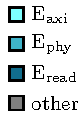
\includegraphics{assets/legend.pdf}
    }
    \hfill
    \subcaptionbox{PCM\label{fig:sunburst_avg_conf_proc_pcm}}{
        \import{assets/power_analysis}{pre}
\begin{tikzpicture}
    \pie[
        radius=2.3,
        text=pin,
        hide number,
    ]{
        1.2/1.2\%,
        2.6/2.6\%,
        5.0/5.0\%,
        3.0/3.0\%
    }
    \pie[
        radius=2.3,
        hide number,
        color={gray, bluehue2, bluehue4, bluehue6},
        before number=\printonlylargeenough{2},
        after number=\ifprintnumber\%\fi
    ]{
        1.2/,
        2.6/,
        5.0/,
        3.0/
    }
    \pie[
        radius=1.8,
        text=inside,
        color={blue!60, red!60},
    ]{
        11.8/$\econf$,
        88.2/$\eproc$
    }
\end{tikzpicture}

    }
    \caption{Average energy consumption distribution of the models listed in \cref{tab:example_models_stats}}
    \label{fig:example_models_avg_conf_proc}
\end{figure}

Ideally, the energy consumption of the configuration of a model should be as small as possible.
In \cref{ch:7}, we explore techniques for increasing configuration efficiency.
    
These findings provide valuable insights into the dynamic energy consumption of LPDDR5X and PCM across different models, highlighting the potential of PCM for reduced configuration energy.
However, it is important to emphasize that this analysis focused solely on dynamic energy, which is the energy consumed during active operation.
To gain a complete understanding of the energy efficiency of these technologies, further investigation into static energy consumption is necessary.
